\documentclass[12pt, a4paper, oneside]{ctexart}
\usepackage{amsmath, amsthm, amssymb, bm, color, graphicx, geometry, hyperref, mathrsfs,extarrows, braket, booktabs, array}
\setmainfont{Times New Roman}  % 设置英文字体
\setsansfont{Calibri}
\setmonofont{Consolas}

\linespread{1.4}
%\geometry{left=2.54cm,right=2.54cm,top=3.18cm,bottom=3.18cm}
\geometry{left=1.84cm,right=1.84cm,top=2.18cm,bottom=2.18cm}
\newenvironment{problem}{\par\noindent\textbf{题目. }}{\bigskip\par}
\newenvironment{solution}{\par\noindent\textbf{解答. }}{\bigskip\par}
\newenvironment{note}{\par\noindent\textbf{注记. }}{\bigskip\par}

\everymath{\displaystyle} % 默认全部行间公式
\DeclareMathOperator*\uplim{\overline{lim}} % 定义上极限 \uplim_{}
\DeclareMathOperator*\lowlim{\underline{lim}} % 定义下极限 \lowlim_{}
\let\leq=\leqslant % 将全部leq变为leqslant
\let\geq=\geqslant % geq同理

% 一些宏定义
\def\bd{\boldsymbol}    % 加粗(向量) boldsymbol
\def\disp{\displaystyle}% 使用行间公式 displaystyle(默认)
\def\tsty{\textstyle}   % 使用行内公式 textstyle
\def\sign{\text{sign}}  % sign function
\def\wtd{\widetilde}    % 宽波浪线 widetilde
\def\R{\mathbb{R}}      % Real number
\def\Q{\mathbb{Q}}      % Rational number (Quotient)
\def\C{\mathbb{C}}      % Complex number
\def\d{\mathrm{d}}      % differential operator
\def\P{\textbf{P}}      % Probability
\def\E{\textbf{E}}      % Exception
\def\var{\textbf{Var}}  % variance
\def\cov{\textbf{Cov}}  % covariance
\def\e{\mathrm{e}}      % Euler's number
\def\i{\mathrm{i}}      % imaginary number
\def\L{\mathcal{L}}     % Loss function
\def\wdh{\widehat}      % 宽帽子 widehat
\def\ol{\overline}      % 上横线 overline
\def\ul{\underline}     % 下横线 underline
\def\add{\vspace{0.5ex}}  % 增加行间距
\def\del{\vspace{-3.5ex}}  % 减少行间距

% 基本信息
\newcommand{\RQ}{\today} % 日期
\newcommand{\km}{概率论} % 科目
\newcommand{\bj}{强基数学002} % 班级
\newcommand{\xm}{吴天阳} % 姓名
\newcommand{\xh}{2204210460} % 学号

\begin{document}

%\pagestyle{empty}
\pagestyle{plain}
\vspace*{-15ex}
\centerline{\begin{tabular}{*5{c}}
    \parbox[t]{0.25\linewidth}{\begin{center}\textbf{日期}\\ \large \textcolor{blue}{\RQ}\end{center}} 
    & \parbox[t]{0.2\linewidth}{\begin{center}\textbf{科目}\\ \large \textcolor{blue}{\km}\end{center}}
    & \parbox[t]{0.2\linewidth}{\begin{center}\textbf{班级}\\ \large \textcolor{blue}{\bj}\end{center}}
    & \parbox[t]{0.1\linewidth}{\begin{center}\textbf{姓名}\\ \large \textcolor{blue}{\xm}\end{center}}
    & \parbox[t]{0.15\linewidth}{\begin{center}\textbf{学号}\\ \large \textcolor{blue}{\xh}\end{center}} \\ \hline
\end{tabular}}
\vspace*{4ex}

% 正文部分
\paragraph{习题 5.1}\del
\paragraph{1.}甲、乙两队进行篮球比赛, 若有一队胜$4$场比赛就结束, 假设甲、乙两队在每场比赛中获胜的概率都是$\frac{1}{2}$, 求所需比赛的场数的数学期望.
\begin{solution}
    设$X$为所需比赛的场数, 由题意可知$\P(X = k) = b\left(4;k,\frac{1}{2}\right) = \binom{k}{4}\left(\frac{1}{2}\right)^k$, 于是
    \begin{equation*}
        \E X = 4\cdot\left(\frac{1}{2}\right)^4+5\cdot\binom{5}{4}\left(\frac{1}{2}\right)^5+6\cdot\binom{6}{4}\left(\frac{1}{2}\right)^6+7\cdot\binom{7}{4}\left(\frac{1}{2}\right)^7 \approx 4.35156
    \end{equation*}
\end{solution}\del
\paragraph{3.}假设公共汽车起点站于每时的$10$分、$30$分、$50$分发车, 某乘客不知发车时间, 在每一小时内任一时刻到达车站是随机的, 求乘客到达车站等车时间的数学期望.
\begin{solution}
    设$S$为乘客到达车站等车时间, $X$为乘客到达车站的事件, 不妨将每个小时从$10$分钟开始计算, 则$10\leq X\leq 70$, 则有如下关系式:
    \begin{equation*}
        S = \begin{cases}
            30 - X,&\quad 10\leq X < 30,\\
            50 - X,&\quad 30\leq X < 50,\\
            70 - X,&\quad 50\leq X\leq 70.
        \end{cases}
    \end{equation*}
    且$\P(x) = \frac{1}{60}$, 于是
    \begin{align*}
        \E S = \int_{10}^{70}y\,\d F(S) =&\ \int_{10}^{30}(30-x)\P(x)\,\d x+\int_{30}^{50}(50-x)\P(x)\,\d x+\int_{50}^{70}(70-x)\P(x)\,\d x \\
        =&\ 3\int_{10}^{30}\frac{(30-x)}{60}\,\d x= \frac{(60-x)x}{40}\biggl|_{10}^{30} = 10
    \end{align*}
\end{solution}
\paragraph{8.}设$X_1,\cdots, X_n$为独立同分布的$U(0,1)$随机变量, 求
\begin{equation*}
    \E\min\{X_1,\cdots, X_n\}\qquad\text{和}\qquad\E\max\{X_1,\cdots, X_n\}.
\end{equation*}
\begin{solution}
    设$Y_1 = \min\{X_1,\cdots, X_n\},\ Y_2 = \max\{X_1,\cdots, X_n\}$, 则$F_{Y_1}(x) = 1-(1-x)^n,\ F_{Y_2}(x) = x^n$, 所以$\P_{Y_1}(x) = n(1-x)^{n-1},\ \P_{Y_2}(x) = nx^{n-1}$, 于是
    \begin{align*}
        \E Y_1 =&\ \int_0^1nx(1-x)^{n-1}\,dx = n\sum_{k=0}^{n-1}(-1)^k\binom{n-1}{k}\int_0^1x^{k+1}\,\d x = n\sum_{k=0}^{n-1}(-1)^k\binom{n-1}{k}\frac{1}{k+2},\\
        \E Y_2 =&\ \int_0^1nx^n\,\d x = \frac{n}{n+1}.
    \end{align*}
\end{solution}
\paragraph{9.}设$X_1,X_2$相互独立, 均服从$\mathcal{N}(a, \sigma^2)$, 试证:
\begin{equation*}
    \E\max\{X_1, X_2\} = a+\frac{\sigma}{\sqrt{\pi}}.
\end{equation*}
\begin{proof}
    由于$\E \max\{X_1,X_2\} = \E\left(\frac{X_1+X_2+|X_1-X_2|}{2}\right) = a + \frac{1}{2}\E|X_1-X_2|$, 又由于$X_1-X_2\sim\mathcal{N}(0,2\sigma^2)$, 于是$p_{X_1-X_2}(x)=  \frac{1}{2\sqrt{\pi}\sigma}\exp\left\{\-\frac{x^2}{4\sigma^2}\right\}$, 则
    \begin{equation*}
        \E|X_1-X_2| = \frac{1}{2\sqrt{\pi}\sigma}\int_0^{\infty}2xe^{-\frac{x^2}{2\sigma^2}}\,\d x = \frac{2\sigma}{\sqrt{\pi}},
    \end{equation*}
    所以$\E\max\{X_1,X_2\} = a+\frac{1}{2}\,\frac{2\sigma}{\sqrt{\pi}} = a+\frac{\sigma}{\sqrt{\pi}}$.
\end{proof}
\paragraph{13.}设随机变量$X$取任意正整数的概率依几何级数减少. 式选择级数的首项$a$及公比$q$, 使随机变量的期望等于$10$, 并在此条件下, 计算$X$不大于$10$的概率.
\begin{solution}
    由题可知$\P(X=k) = aq^{k-1},\ (k\geq 1)$, 于是$\E X = \sum_{k=1}^\infty k\cdot ap^{k-1} = 10$, 且$\sum_{k=1}^\infty ap^{k-1} = 1$, 则$\frac{a}{1-p} = 1\Rightarrow a= 1-p$. 于是$(1-p)\sum_{k=1}^\infty kp^{k-1} = 10$, 由于
    \begin{equation*}
        \sum_{k=1}^\infty kp^{k-1} = \sum_{k=1}^\infty(p^k)' = \left(\sum_{k=1}^\infty p^k\right)' = \left(\frac{p}{1-p}\right)' = \frac{1}{(1-p)^2},
    \end{equation*}
    所以$\frac{1-p}{(1-p)^2}=\frac{1}{1-p} = 10$, 故$p = \frac{9}{10}, a = \frac{1}{10}$.
    \begin{equation*}
        \P(X\leq 10) = a(1+q^1+\cdots + q^9) = \frac{1}{10}\sum_{k=0}^9(\frac{9}{10})^k = 1-\left(\frac{9}{10}\right)^{10}.
    \end{equation*}
\end{solution}\del
\paragraph{14.}在长为$a$的线段上相互独立地选取$n$个点, 求相距最远的两点间距离的期望.
\begin{solution}
    $n$个点将线段分为的$n+1$段, 长度分别令为$X_0, X_1,\cdots, X_n$, 且$\E(X_0+X_1+\cdots+X_n) = a$, 有对称性可知, $X_i\ (i=1,2,\cdots, n)$具有相同的分布律, 所以$\E(X_i) = \frac{a}{n+1}\ (i=1,2,\cdots, n)$, 因此
    \begin{equation*}
        \E(X_1+\cdots+X_{n-1}) = (n-1)\E(X_i) = \frac{n-1}{n+1}a.
    \end{equation*}
\end{solution}\del
\paragraph{19.}设$F(x)$为某非负随机变量的分布函数, 试证: 对任意$s > 0$有
\begin{equation*}
    \int_0^\infty x^s\,\d F(x) = s\int_0^{\infty}x^{s-1}(1-F(x))\,\d x.
\end{equation*}
\begin{proof}
    \begin{align*}
        \int_0^\infty x^s\,\d F(x) =&\ -\int_0^{\infty}x^s\,\d(1-F(x)) = -x^s(1-F(x))\biggl|_0^{\infty}+\int_0^\infty s x^{s-1}(1-F(x))\,\d x\\ =&\ s\int_0^\infty x^{s-1}(1-F(x))\,\d x.
    \end{align*}
\end{proof}
\paragraph{26.}现有$n$个袋子, 各装有$a$个白球$b$个黑球, 先从第一个袋子中摸出一球, 几下颜色后把它放入第二个袋子中, 再从第二个袋子中摸出一球, 记下颜色后把它放入第三个袋子中, 照这样的办法一直摸下去, 最后从第$n$个袋子摸出一球并记下颜色, 若在这$n$次模球中所摸得的白球的总数为$S_n$, 试求$\E S_n$.
\begin{solution}
    设$X_i$为第$i$次摸球的结果, 记$X_i=0$摸出白球, $X_i = 1$摸出黑球, 则
    \begin{align*}
        &\ \P(X_1 = 0) = \frac{a}{a+b},\qquad \P(X_2 = 0) = \frac{a+\P(X_1 = 0)}{a+b+1} = \frac{a + \frac{a}{a+b}}{a+b+1} = \frac{a}{a+b}\\
        &\ \P(X_i = 0) = \frac{a+\P(X_i = 0)}{a+b+1} = \frac{a}{a+b}.
    \end{align*}
    所以
    \begin{equation*}
        \E S_n = \sum_{i=1}^n1\cdot \P(X_i = 0) = \frac{an}{a+b}.
    \end{equation*}
\end{solution}\del
\paragraph{28.}将一枚硬币连续抛掷$n$次, 假设各次抛掷相互独立进行, 每次抛出正面的概率都是$p\ (0 < p < 1)$. 如果相继抛掷的两次所抛出的面不同, 则称出现一次转换. 例如: 对$n=5$, 若抛掷结果为“正正反正反”, 则称其中出现$3$次转换. 以$X$表示$n$次抛掷中所出现的转换次数, 求$\E X$.
\begin{solution}
    设$X_i$为第$i$次抛掷的结果, 记$X_i = 1$为正面, $X_i = 0$为反面. 设$Y_i$为第$i$次抛掷结果和$i-1$次抛掷结果不同的事件, 则$\P(X_i = 1) = p,\ \P(X_i = 0 ) =1-p$, 于是
    \begin{equation*}
        \P(Y_i) = \P(X_i = 1)\P(X_{i-1} = 0)+\P(X_i = 0)\P(X_{i-1} = 1) = 2p(1-p),
    \end{equation*}
    所以
    \begin{equation*}
        \E X = \sum_{i=2}^n\P(Y_i) = 2(n-1)p(1-p).
    \end{equation*}
\end{solution}\del
\paragraph{29.}设随机变量$X$的密度函数为
\begin{equation*}
    p(x) = \begin{cases}
        \frac{1}{2}e^x,&\quad x\leq 0,\add\\
        \frac{1}{2}e^{-x}, &\qquad x > 0,
    \end{cases}
\end{equation*}
求$|X|$的数学期望和方差.

\begin{solution}
    由题意可知, $p(x) = \frac{1}{2}e^{-|x|}$, 考虑$|X|$的矩母函数
    \begin{equation*}
        f(t) = \E e^{t|X|} = \int_{-\infty}^\infty e^{t|x|}\cdot \frac{1}{2}e^{-|x|}\,\d x = \int_0^{\infty}e^{(t-1)x}\,\d x = \frac{1}{1-t},
    \end{equation*}
    所以$\E |X| = f'(0) = 1,\ \E |X|^2 = f''(0) = 2$, 于是$\var |X| = \E |X|^2-(\E X)^2 = 1$.
\end{solution}
\paragraph{30.}设随机变量$X$的密度函数为
\begin{equation*}
    p_X(x) = 2(x-1),\quad 1 < x < 2.
\end{equation*}
求$Y=e^X$与$Z =\frac{1}{X}$的数学期望和方差.
\begin{solution}
    \begin{align*}
        &\ \E Y = \int_1^22(x-1)e^x\,\d x = 2e,\quad \E Y^2 = \int_1^2 2(x-1)e^{2x}\,\d x = \frac{1}{2}(e^4+e^2)\\
        &\ \var Y = \E Y^2 - (\E Y)^2 = \frac{1}{2}e^2(e^2 - 7).\\
        &\ \E Z = \int_1^2\frac{2(x-1)}{x}\,\d x = 2(1-\log 2),\quad \E Z^2 = \int_1^2\frac{2(x-1)}{x^2}\,\d x = 2(\log 2+\frac{1}{2})\\
        &\ \var Z = \E Z^2 - (\E Z)^2 = 10\log 2-4\log ^2 2-3.
    \end{align*}
\end{solution}\del\del
\paragraph{习题 5.2}
\paragraph{2.}设$X$与$Y$为相互独立的$U(0,1)$随机变量, 证明: 对任何$a>0$, 都有
\begin{equation*}
    \E|X-Y|^a = \frac{2}{(a+1)(a+2)}.
\end{equation*}
\begin{solution}\del
    \begin{align*}
        \E|X-Y|^a =&\ \int_0^1 \E|X-Y|^a\,\d y = \int_0^1\,\d y\int_0^1|x-y|^a\,\d x\\
        =&\ \int_0^1\left(\int_y^1(x-y)^a\,\d x+\int_0^y(y-x)^a\,\d x\right)a\,\d y\\
        =&\ \int_0^1\frac{(1-y)^{a+1}+y^{a+1}}{a+1}\,\d y\\
        =&\ \frac{2}{(a+1)(a+2)}.
    \end{align*}
\end{solution}\del\del
\paragraph{4.}罐中有一个黑球, 每次从中取出一个求, 并随机放入一个新球, 新球为黑球的概率为$p\ (0<p<1)$, 为白球的概率为$1-p$, 一直到罐中没有黑球为止. 将所进行的取球次数记为$X$, 求$\E X$.\add
\begin{solution}
    由于$X$服从$1-p$的几何分布, 所以$\E X = \frac{1}{1-p}$.
\end{solution}
\paragraph{9.}设$g(x)$为任一可测函数, 证明: 若下列期望均存在, 则
\begin{equation*}
    \E[\E(Y|X)g(X)] = \E[Yg(X)].
\end{equation*}
\begin{proof}\ \del
    \begin{align*}
        \E(\E(Y|X)g(X)) =&\ \int_{-\infty}^\infty\E(Y|X = x)g(x)p_1(x)\,\d x\\
        =&\ \int_{-\infty}^\infty g(x)p_1(x)\,\d x\int_{-\infty}^\infty y\P(Y=y|X=x)\,\d y\\
        =&\ \int_{-\infty}^\infty p_1(x)\,\d x\int_{-\infty}^\infty yg(x)\P(Y=y|X=x)\,\d y\\
        =&\ \int_{-\infty}^\infty p_1(x)\E(Yg(X)|X= x)\,\d x = \E(Yg(X)).
    \end{align*}
\end{proof}\del
\paragraph{10.}设随机向量$(X, Y)$的密度函数为$p(x, y) = cx(y-x)e^{-y},\ 0<x<y<\infty$. 试求常数$c$, 及条件期望$\E(X|Y)$和$\E(Y|X)$.
\begin{solution}
    \begin{align*}
        \int_0^{\infty}\,\d x\int_x^\infty cx(y-x)e^{-y}\,\d y = \int_0^{\infty}\,\d y\int_0^y cx(y-x)e^{-y}\,\d x = \int_0^\infty \frac{c}{6}y^3e^{-y}\,\d y = c = 1.
    \end{align*}
    则$p(x, y) = x(y-x)e^{-y}\quad(0<x<y<\infty)$, 于是
    \begin{align*}
        \E(X|Y) =&\ \int_0^\infty \E(X|Y = y)p_2(y)\,\d y = \int_0^\infty p_2(y)\,\d y \int_0^y \P(X=x|Y=y)x\,\d x\\
        =&\ \int_0^\infty\,\d y\int_0^yx^2(y-x)e^{-y}\,\d x = \int_0^{\infty}\frac{1}{12}y^4e^{-y}\,\d y = 2,\\
        \E(Y|X)=&\ \int_0^\infty\E(Y|X= x)p_1(x)\,\d x = \int_0^\infty p_1(x)\,\d x\int_x^{\infty}\P(Y=y|X=x)y\,\d y\\
        =&\ \int_0^\infty \,\d x\int_x^\infty \left(xy^2e^{-y}-x^2ye^{-y}\right)\,\d y = \int_0^{\infty}(x^2+2x)e^{-x}\,\d x = 4.
    \end{align*}
\end{solution}\del\del
\paragraph{11.}设随机变量$X, Y$和$Z$相互独立, 且分别服从参数为$\lambda,\mu$和$\nu$的指数分布, 试求$\P(X<Y<Z)$.
\begin{solution}\ \del
    \begin{equation*}
        \P(X<Y<Z) = \int_0^{\infty}\lambda e^{-\lambda x}\,\d x\int_x^\infty \mu e^{-\mu y}\,\d y\int_y^{\infty}\nu e^{-\nu z}\,\d z = \frac{\lambda\mu}{(\mu+\nu)(\lambda+\mu+\nu)}.
    \end{equation*}
\end{solution}\del\del
\clearpage
\paragraph{习题5.3}
\paragraph{1.}设随机变量$X_1,X_2,\cdots,X_{m+n}\ (n > m)$是独立的, 有相同的分布并且有有限的方差, 试求$S = X_1+\cdots + X_n$与$T = X_{m+1}+X_{m+2}+\cdots+X_{m+n}$两和之间的相关系数.
\begin{solution}
    由于$X_i$之间是相互独立的, 所以它们也是不相关的, 又由于它们满足相同的分布, 所以$\var(S) = \var(T) = n\var(X_1)$, 由于
    \begin{equation*}
        \begin{aligned}
            \cov(S, T) =&\ \cov \left(\sum_{i=1}^n X_i,\sum_{j=1}^n X_{m+j}\right) = \sum_{i=1}^n\sum_{j=1}^n\cov\left(X_i, X_{m+j}\right)\\
            =&\ \sum_{i=m+1}^n\cov(X_i, X_i) = (n-m)\cov (X_1, X_1) = (n-m)\var(x).
        \end{aligned}
    \end{equation*}
    所以相关系数$r = \frac{\cov(S, T)}{\sqrt{\var(S)}\sqrt{\var(T)}} = \frac{n-m}{n}.$
\end{solution}
\paragraph{5.}设$Y_1=aX_1+b,\ Y_2 = cX_2+d$, 其中$ac > 0$. 证明$Y_1, Y_2$的相关系数等于$X_1, X_2$的相关系数.
\begin{proof}
    由于
    \begin{align*}
        \cov(Y_1, Y_2) =&\ \E(acX_1X_2+adX_1+bcX_2+cd) - \E(aX_1+c)\E(cX_2+d)\\
        =&\ ac[\E(X_1X_2)-\E(X_1)\E(X_2)],\\
        \var(Y_1) =&\ \var(aX_1+b) = \var(aX_1) = a^2\var(X_1),\\
        \var(Y_2) =&\ \var(aX_2+b) = \var(aX_2) = a^2\var(X_2).
    \end{align*}
    由于$ac >0$, 则$|ac| = ac$, 于是
    \begin{equation*}
        r_{Y_1,Y_2} = \frac{\cov(Y_1,Y_2)}{\sqrt{\var(Y_1)}\sqrt{\var(Y_2)}} = \frac{ac[\E(X_1X_2)-\E(X_1)\E(X_2)]}{|ac|\sqrt{\var(X_1)}\sqrt{\var(X_1)}} = \frac{\cov(X_1,X_2)}{\sqrt{\var(X_1)}\sqrt{\var(X_2)}} = r_{X_1,X_2}.
    \end{equation*}
\end{proof}
\paragraph{7.}若$X, Y$服从二维正态分布, $\E X = a,\ \var X = 1,\ \E Y = b, \var Y = 1$, 证明: $X$与$Y$的相关系数$r$等于$\cos q\pi$, 其中$q = \P((X-a)(Y-b) < 0)$.
\paragraph{9.}袋中由编号$1$至$n$的$n$张卡片, 现从中任取出$m(m\leq n)$张. 试对(1)有放回; (2)不放回两情况求$m$张卡片上编号之和的方差.
\begin{solution}
    设$X_i\ (i=1,2,\cdots, m)$为第$i$次取卡时卡片的编号, 则
    (1) 有放回时
    \begin{align*}
        \E(X_i) =&\ \sum_{i=1}^n\frac{i}{n} = \frac{n(n+1)}{2n},\quad \E(X_i^2) = \sum_{i=1}^n\frac{i^2}{n} = \frac{n(n+1)(2n+1)}{6n},\\
        \var(X_i) =&\ \E(X_i^2) - (\E(X_i))^2 = \frac{n(n+1)(n-1)}{3n}.
    \end{align*}
    由于$X_i$两两之间是不相关的, 所以$\cov\left(\sum_{i=1}^{k-1}X_i, X_k\right) = \sum_{i=1}^{k-1}\cov(X_i, X_k) = 0\ (k=2, 3,\cdots, m)$, 于是
    \begin{equation*}
        \var(\sum_{i=1}^m X_i) = \sum_{i=1}^m\var(X_i) = \frac{mn(n+1)(n-1)}{3n}.
    \end{equation*}

    (2)无放回, 设$X_i$为编号为$i$的卡片的示性变量, 则$S = \sum_{i=1}^n ix_i$, 
    \begin{equation*}
        \var(S) = \sum_{i=1}^ni^2\var(X_i) +\sum_{1\leq i < j\leq n}ij\cov(X_i, X_j),\\
    \end{equation*}
    由于$\P(X_i = 1)=\frac{\binom{n-1}{m-1}}{\binom{n}{m}}$, 且$X_i = X_i^2$, 则
    \begin{align*}
        \var(X_i) =&\ \E(X_i^2)-(\E(X_i))^2 = \E(X_i) - (\E(X_i))^2 = \frac{\binom{n-1}{m-1}}{\binom{n}{m}}-\left(\frac{\binom{n-1}{m-1}}{\binom{n}{m}}\right)^2,\\
        \cov(X_i,X_j) =&\ \E(X_iX_j)-\E(X_i)\E(X_j),\\
        \E(X_iX_j) =&\ \E(X_i|X_j=1) = \frac{\binom{n-2}{n-2}}{\binom{n-1}{m-1}}\,\frac{\binom{n-1}{m-1}}{\binom{n}{m}}=\frac{\binom{n-2}{m-2}}{\binom{n}{m}},
    \end{align*}
    综上
    \begin{equation*}
        \var(S) = \sum_{i=1}^ni^2\left(\frac{\binom{n-1}{m-1}}{\binom{n}{m}}-\left(\frac{\binom{n-1}{m-1}}{\binom{n}{m}}\right)^2\right)+\sum_{1\leq i<j\leq n}ij\left(\frac{\binom{n-2}{m-2}}{\binom{n}{m}}-\left(\frac{\binom{n-1}{m-1}}{\binom{n}{m}}\right)^2\right).
    \end{equation*}
\end{solution}
\paragraph{13.}设$\E X^2 < \infty$, $a$是实数, 令
\begin{equation*}
    Y = \begin{cases}
        X,&\quad X\leq a,\\
        a,&\quad X > a,
    \end{cases}
\end{equation*}
证明: $\var Y\leq\var X$.
\paragraph{15.}设随机变量$X$与$Y$独立同分布, 且其分布函数$F(x)$为连续函数. 若$\E X$存在, 试证明: \begin{equation*}
    \E|X-Y| = 4\cov(X,F(X)).
\end{equation*}
\begin{proof}
    \begin{align*}
        \E(X-Y) =&\ \int_{-\infty}^\infty\int_{-\infty}^\infty |x-y|\,\d F(x, y)\\
        \xlongequal{X, Y\text{独立}}&\ \int_{-\infty}^\infty\int_{-\infty}^\infty|x-y|\,\d F(x)\,\d F(y)\\
        =&\ \int_{-\infty}^\infty\,\d F(x)\int_{-\infty}^x(x-y)\,\d F(y)+\int_{-\infty}^\infty\,\d F(x)\int_{x}^\infty(y-x)\,\d F(y)\\
        =&\ \int_{-\infty}^\infty x\,\d F(x)\int_{-\infty}^x\,\d F(y) - \int_{-\infty}^\infty\,\d F(x)\int_{-\infty}^x y\,\d F(y)\\
        &\ +\int_{-\infty}^\infty \,\d F(x)\int_{x}^\infty y\,\d F(y)-\int_{-\infty}^\infty x\,\d F(x)\int_{x}^\infty\,\d F(y)\\
        \xlongequal[\text{交换积分顺序}]{X,Y\text{同分布}}&\ \int_{-\infty}^\infty xF(x)\,\d F(x) - \int_{-\infty}^\infty y\,\d F(y)\int_{y}^\infty \,\d F(x)\\
        &\ +\int_{-\infty}^\infty y\,\d F(y)\int_{-\infty}^y \,\d F(x)-\int_{-\infty}^\infty x(1-F(x))\,\d F(x)\\
        =&\ \int_{-\infty}^\infty xF(x)\,\d F(x) - \int_{-\infty}^\infty y(1-F(y))\,\d F(y)\\
        &\ +\int_{-\infty}^\infty yF(y)\,\d F(y) - \int_{-\infty}^\infty x(1-F(x))\,\d F(x)\\
        \xlongequal{X,Y\text{同分布}}&\ 4\int_{-\infty}^\infty xF(x)\,\d F(x) - 2\int_{-\infty}^\infty x\,\d F(x)\\
        =&\ 4\E(XF(X)) - 2\E(X)\\
        \xlongequal[\E(F(X)) = \frac{1}{2}]{F(X)\sim U(0,1)}&\ 4\E(XF(X)) - 4\E(X)\E(F(X)) = 4\cov(X, F(X)).
    \end{align*}
\end{proof}
\paragraph{习题5.4}
\paragraph{1.}求Pascal分布$f(k;r,p)$的特征函数, 并用特征函数求其期望.
\begin{solution}
    Pascal分布即为负二项分布, 表示在第$k+r$次Bernoulli试验中, 恰好成功了$r$次, 则第$k+r$次试验必定成功, 于是
    \begin{equation*}
        \P(X = r+k) = p\binom{r+k-1}{k}p^{r-1}q^k
    \end{equation*}
    且
    \begin{align*}
        &\ \sum_{k=0}^\infty p\binom{r+k-1}{k}p^{r-1}q^k = 1\\
        \Rightarrow&\ \sum_{k=0}^\infty \binom{r+k-1}{k}q^k = \frac{1}{p^r} = \frac{1}{(1-q)^r}.
    \end{align*}
    所以, 特征函数为
    \begin{align*}
        f(t) =&\ \sum_{k=0}^\infty p\binom{r+k-1}{k}p^{r-1}q^k\e^{it(r+k)}\\
        =&\ p^r\e^{\i tr}\sum_{k=0}^\infty\binom{r+k-1}{k}\left(q\e^{\i t}\right)^k = \left(\frac{p\e^{\i t}}{1-q\e^{\i t}}\right)^r.
    \end{align*}
    进一步, Pascal分布的期望为
    \begin{align*}
        \E X = \frac{f'(0)}{i} = r\left(1+\frac{q}{p}\right) = \frac{r}{p}\ .
    \end{align*}
\end{solution}\del\del
\paragraph{2.}求Gamma分布$\Gamma(\lambda, r)$的特征函数, 并用特征函数求其$k$阶原点矩$m_k$.
\begin{solution}
    设$X\sim \Gamma(\lambda, r)$, 则$p(x) = \frac{\lambda^r}{\Gamma(r)}x^{r-1}e^{-\lambda x}$, 于是
    \begin{align*}
        f(t)=&\ \E\e^{\i tx} = \int_0^\infty \frac{\lambda^r}{\Gamma(r)}x^{r-1}\e^{-\lambda x}e^{-\i tx}\,\d x\\
        =&\ \left(1-\frac{\i t}{\lambda}\right)^{-r}\int_0^\infty \frac{\left(\lambda\left(1-\frac{\i t}{\lambda}\right)\right)^r}{\Gamma(r)}x^{r-1}\e^{-\lambda\left(1-\frac{\i t}{\lambda}\right)x}\,\d x\\
        =&\ \left(1-\frac{\i t}{\lambda}\right)^{-r}.
    \end{align*}
    则$f^{(k)}(t) = \frac{\i^kr(r+1)\cdots(r+k-1)}{\lambda^k}\left(1-\frac{\i t}{\lambda}\right)^{-r-t}$, 所以
    \begin{equation*}
        \E X^k = \frac{f^{(k)}(t)}{i^k} = \frac{r(r+1)\cdots(r+k-1)}{\lambda^k}.
    \end{equation*}
\end{solution}\del\del
\paragraph{5.}设$g(u) = 1-|u|,\ |u| < 1$.

(1) 求以$g(x)$为密度函数的分布的特征函数;

(2) 用反演公式求以$g(t)$为特征函数的分布的密度函数.
\begin{solution}
    (1) 特征函数为
    \begin{align*}
        f(t) =&\ \int_{-\infty}^\infty g(x)\e^{\i tx}\,\d x\\
        =&\ \int_{-1}^0(1+x)\e^{\i tx}\,\d x +\int_0^1(1-x)\e^{\i tx}\,\d x\\
        =&\ \frac{1}{\i t}(-2e^{-\i t}+\frac{1}{\i t}(e^{\i t}+e^{-\i t}-2)).
    \end{align*}

    (2) 由反演公式知, 密度函数为
    \begin{align*}
        p(x) =&\ \frac{1}{2\pi}\int_{-1}^{1}(1-|t|)e^{-\i tx}\,\d t\\
        =&\ \frac{1}{2\pi}\int_{-1}^0(1+t)\e^{-\i tx}\,\d t+\frac{1}{2\pi}\int_0^1(1-t)\e^{-\i tx}\,\d t\\
        =&\ \frac{1}{2\pi}\left(\frac{1}{-\i t}\left(-2\e^{\i t}+\frac{1}{-\i t}\left(\e^{-\i t}+\e^{\i t}-2\right)\right)\right).
    \end{align*}
\end{solution}

% 下面给一些功能的写法
\iffalse
% 图片模板
\centerline{
    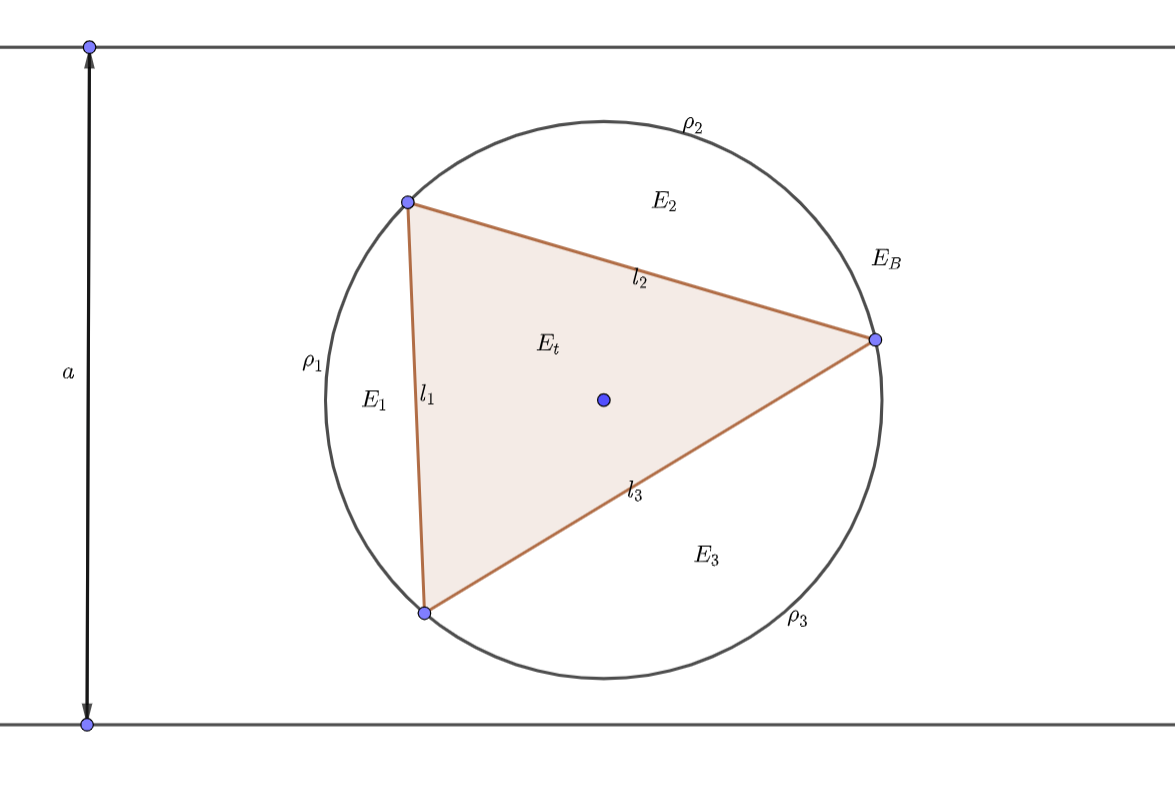
\includegraphics[width=0.8\textwidth]{figure.png}
}
% 表格模板
\renewcommand\arraystretch{0.8} % 设置表格高度为原来的0.8倍
\begin{table}[!htbp] % table标准
    \centering % 表格居中
    \begin{tabular}{p{1cm}<{\centering}p{1cm}<{\centering}p{3cm}<{\centering}p{5cm}<{\centering}} % 设置表格宽度
    %\begin{tabular}{cccc}
        \toprule
        $x_i$ & $f[x_1]$ & $f[x_i,x_{i+1}]$ & $f[x_i,x_{i+1},x_{i+2}]$ \\
        \midrule
        $x_0$ & $f(x_0)$ &                  &                          \\
        $x_0$ & $f(x_0)$ & $f'(x_0)$        &                          \\
        $x_0$ & $f(x_1)$ & $\frac{f(x_1)-f(x_0)}{x_1-x_0}$ & $\frac{f(x_1)-f(x_0)}{(x_1-x_0)^2}-\frac{f'(x_0)}{x_1-x_0}$\\
        \bottomrule
    \end{tabular}
\end{table}

\def\Log{\text{Log}} % 一个简单的宏定义
$\Log$ % 调用方法
\fi

\end{document}